% Source of the journal-format manuscript of article 2 (Izvestiya RAN, Ser. Geogr., rules of 17.11.2025).
% Citation placeholders and the two bibliography markers are expanded by
% tools/build_article2_journal.py into article2_v3.tex (plain-text author-year citations).
\documentclass[12pt,a4paper]{article}
\usepackage[a4paper,top=2cm,bottom=2cm,left=3cm,right=1.5cm]{geometry}
\usepackage{iftex}
\ifPDFTeX
  \usepackage[T2A]{fontenc}
  \usepackage[utf8]{inputenc}
  \usepackage[russian]{babel}
\else
  \usepackage{fontspec}
  \usepackage{polyglossia}
  \setdefaultlanguage{russian}
  \setotherlanguage{english}
  \defaultfontfeatures{Ligatures=TeX}
  \IfFontExistsTF{Times New Roman}{%
    \setmainfont{Times New Roman}\newfontfamily\cyrillicfont{Times New Roman}%
  }{%
    \IfFontExistsTF{Liberation Serif}{%
      \setmainfont{Liberation Serif}\newfontfamily\cyrillicfont{Liberation Serif}%
    }{\setmainfont{CMU Serif}\newfontfamily\cyrillicfont{CMU Serif}}%
  }
\fi
\usepackage{setspace}
\usepackage{mathtools,amssymb}
\usepackage{graphicx}
\usepackage{booktabs}
\usepackage{array}
\usepackage{caption}
\captionsetup{labelsep=period,font=normalsize,justification=raggedright,singlelinecheck=false}
\usepackage{titlesec}
\titleformat{\section}{\normalfont\bfseries\centering}{}{0pt}{}
\titleformat{\subsection}{\normalfont\itshape}{}{0pt}{}
\titlespacing*{\section}{0pt}{18pt}{6pt}
\titlespacing*{\subsection}{0pt}{12pt}{3pt}
\usepackage[unicode,hidelinks]{hyperref}
\setlength{\parindent}{1.25cm}
\setlength{\emergencystretch}{3em}
\hyphenpenalty=10000 \exhyphenpenalty=10000
\onehalfspacing
\pagestyle{plain}

\begin{document}

\noindent УДК 551.513

\begin{center}
{\large\bfseries География сопряженности иерархических уровней атмосферной циркуляции: планетарная карта, ее факторы и районирование}

\medskip
{\bfseries Н. С. Сотириади\textsuperscript{*}}

Независимый исследователь, Москва, Россия

\textsuperscript{*}E-mail: n.sotiriadi@gmail.com
\end{center}

\begin{singlespace}
\noindent\textbf{Аннотация.} Сопряженность соседних масштабных уровней атмосферной циркуляции -- мера того, насколько размещение мезомасштабной изменчивости предопределено соседним крупным уровнем, -- ранее установлена как устойчивый региональный инвариант. Поставлен географический вопрос: какова планетарная география этого инварианта и чем она определяется. По полю относительного вихря на поверхности 850 гПа (реанализ ERA5) построена глобальная мозаичная карта из 936 ячеек размером около 667 на 700 км между 60$^\circ$ ю.ш. и 60$^\circ$ с.ш. для двух сезонов 2023 г. Карта читается как физико-географическая: максимумы образуют сплошное кольцо штормовых путей Южного океана и штормовые пути северных океанов, минимумы приурочены к очагам глубокой конвекции Амазонии, бассейна Конго и Индонезийского архипелага и к субтропическим муссонным землям. Сопряженность монотонно растет от экватора к умеренным широтам, над океаном выше, чем над сушей, во всех поясах, а в умеренных широтах Южного полушария выше, чем Северного, где штормовой путь разорван материками. Сезонный ход в тропиках следует влажному сезону: сопряженность ниже там и тогда, где активна муссонная конвекция. Атрибуция по заранее заявленным ковариатам подтверждает эту интерпретацию: карта предсказуема вне подгонки ($R^2 = 0.40$--$0.54$, $p = 0.001$), упорядочена одной осью -- активностью штормовых путей, при этом связь двухканальна (штормовая активность повышает сопряженность через спектр, конвекция понижает сверх спектра), а стационарные условия территории восстанавливают 90\% качества предсказания. Свободный модельный расчет воспроизводит карту на 97\% достижимого согласия; воспроизводимый остаток атрибуции географически организован. Предложена типология территорий по организатору циркуляции и уровню сопряженности как основа районирования по устройству межуровневых связей.

\smallskip
\noindent\textbf{Ключевые слова:} штормовые пути, глубокая конвекция, муссон, реанализ, свободный модельный расчет, атрибуция, экзогенные граничные условия, широтная зональность, полушарная асимметрия, типология территорий.
\end{singlespace}

\section{ПОСТАНОВКА ПРОБЛЕМЫ}

Региональная дифференциация атмосферной циркуляции традиционно описывается климатологией ее ведущих организаторов: внетропических штормовых путей -- полос повышенной повторяемости и интенсивности циклонических возмущений умеренных широт \cite{HoskinsValdes1990,Chang2002,HoskinsHodges2005,Shaw2016} -- и режимов глубокой конвекции тропиков и муссонных областей \cite{Houze2004,Feng2021}. В первой статье серии\footnote{Сотириади Н. С. Сопряженность иерархических уровней атмосферной циркуляции как региональный инвариант (первая статья серии; подана в печать). Протоколы, код, данные для воспроизведения и описательный слой настоящей работы открыты в репозитории https://github.com/Theclimateguy/Shroedinger (дата обращения 15.09.2026); постоянный архив версий -- Zenodo, doi: 10.5281/zenodo.19565769; маршрут воспроизведения -- файл reproducibility/article2\_README.md.} к этому описанию добавлена характеристика иного типа: по полю относительного вихря на поверхности 850 гПа построен профиль сопряженности соседних октавных уровней $P$ -- мера того, насколько размещение мезомасштабной изменчивости предопределено соседним крупным уровнем. Показано, что эта величина удовлетворяет операциональному определению инварианта динамики геосистем \cite{Puzachenko1986,Puzachenko2004,Puzachenko2010} в традиции выделения уровней организации регионального климата \cite{Krenke2019}: она устойчива к смене сезона, года, фазы Эль-Ниньо -- Южного колебания (ЭНСО), источника данных \cite{Gelaro2017} и схемы разбиения территории, содержит воспроизводимую информацию сверх спектра поля и воспроизводится в модельном расчете без усвоения наблюдений. Величина $P$ измеряет \emph{пространственную со-организацию} активности соседних уровней; термин “сопряженность” служит кратким обозначением этого факта и не подразумевает ни динамической связи между масштабами, ни переноса энергии -- обе интерпретации отвергнуты в первой статье. Поэтому всюду, где ниже говорится, что режим “повышает” или “понижает” сопряженность, имеется в виду устойчивая статистическая связь заданного знака, а не установленный физический процесс.

Настоящая работа ставит следующий, собственно географический вопрос: какова планетарная география инварианта и чем она определяется -- в каких отношениях его карта находится с известными организаторами циркуляции и с экзогенными условиями территории. Рабочая рамка -- трехзвенная цепь: географическая конфигурация материков, океанов и горных систем задает, где складываются штормовые пути и конвективные режимы; организация этих режимов проявляется в устройстве межуровневых связей; сопряженность уровней есть измеримое выражение последнего звена. Термин “географический” употребляется в трех смыслах: положение (широта, долгота); физико-географические свойства территории (рельеф, соотношение суши и моря, изрезанность берега, температура поверхности океана); тип циркуляционного режима над территорией. Первые два отсылают к условиям, экзогенным по отношению к циркуляции, третий -- к состоянию, складывающемуся вместе с ней. Постановка продолжает отечественную традицию выделения уровней организации геосистем и физико-географического районирования \cite{Sochava1978,Isachenko1991,Bertrand1968} и примыкает к общему для наук о Земле вопросу о масштабе, на котором территория обладает собственной организацией \cite{Simon1962,Levin1992,WuLoucks1995}.

География самих организаторов циркуляции изучена подробно, и это задает точку отсчета для настоящей работы. Положение и интенсивность внетропических штормовых путей определяются бароклинностью нижней тропосферы, которая, в свою очередь, привязана к контрасту суши и океана, к орографии и к фронтам западных пограничных течений; штормовые пути обладают свойством самоподдержания, поскольку сами восстанавливают разрушаемый ими температурный градиент \cite{HoskinsValdes1990}, имеют выраженный сезонный ход с зимним максимумом в Северном полушарии \cite{Chang2002} и слабую сезонность в Южном, где путь непрерывен по кругу широты \cite{Trenberth1991}; современный обзор процессов, задающих их положение и изменчивость, дан в работе \cite{Shaw2016}. Режимы глубокой конвекции столь же географичны: мезомасштабные конвективные системы имеют устойчивую климатологию, привязанную к тропической суше, муссонным областям и Индонезийскому архипелагу \cite{Houze2004,NealeSlingo2003,Feng2021}, а субтропические пустыни и муссоны связаны единым механизмом взаимодействия муссонного нагрева с западным потоком \cite{RodwellHoskins1996}. Ни одна из этих климатологий, однако, не характеризует межуровневую организацию поля: они описывают, где и насколько интенсивны возмущения того или иного масштаба, но не то, насколько согласованно размещены соседние уровни. Между тем именно межуровневая организация определяет, как мезомасштабная изменчивость встраивается в синоптическую: в теории предсказуемости этот канал рассматривается как путь, по которому неопределенность мелких масштабов распространяется на крупные \cite{Zhang2007,RotunnoSnyder2008,Judt2020}, и его сила заведомо различна для бароклинных возмущений штормовых путей и для влажной конвекции. Наследует ли география сопряженности географию организаторов, и если да, то через какие факторы, -- вопрос открытый, и он составляет предмет работы.

Вопрос о географии карты распадается на три конкурирующих объяснения с проверяемыми следствиями; гипотезы и распределение ковариат по ярусам зафиксированы протоколом до вычислений. \emph{H1, экзогенная}: география $P$ определяется стационарными граничными условиями -- рельефом, конфигурацией суши и океана, широтой, полем температуры поверхности океана; следствие -- карта предсказуема по одному ярусу экзогенных условий. \emph{H2, циркуляционная}: география $P$ определяется состоянием циркуляции -- активностью штормовых путей и конвективным режимом; следствие -- ведущие нагрузки принадлежат ярусу характеристик состояния, и связь сохраняется \emph{внутри} климатически однородных областей. \emph{H3, артефактная}: карта -- свойство наблюдательной сети и системы усвоения; следствие -- карта не воспроизводится расчетом без усвоения наблюдений. H1 и H2 не исключают друг друга: если конфигурация задает, где располагаются режимы, оба яруса описывают одну и ту же карту, и содержательным результатом оказывается мера их совместности; проверка потому измеряет вклад каждого яруса по отдельности. Наконец, $P$ заявлен в первой статье как \emph{статичный} инвариант сложившегося режима; отсюда проверяемое следствие: при перестройке режима величина не должна опережать перестройку и превосходить по чувствительности стандартные показатели среднего поля.

Задачи работы: (1) построить глобальную мозаичную карту $P$ и дать ее географическое описание -- широтный ход, полушарную асимметрию, контраст суши и океана, сезонность -- в единстве с атрибуцией по заранее заявленным ковариатам, с отрицательным контролем и контрольной мишенью; (2) описать географию остатка атрибуции; (3) проверить природу карты сопоставлением со свободным модельным расчетом; (4) предложить типологию территорий по организатору циркуляции и уровню сопряженности как основу районирования; (5) замкнуть атрибуцию со стороны времени -- атрибутировать тропический избыток межгодовой изменчивости по заранее названным климатическим индексам и проверить гипотезу статичности.

\section{ДАННЫЕ И МЕТОДИКА ИССЛЕДОВАНИЯ}

Материал -- реанализ ERA5 \cite{Hersbach2020,Soci2024}: составляющие ветра на изобарической поверхности 850 гПа, сетка 0.25$^\circ$, шаг 6 ч, поле относительного вихря -- идентично первой статье. Единица выборки -- ячейка мозаичной карты размером около $667 \times 700$ км, при которой региональная принадлежность служит блокирующим фактором статистики. \emph{Часть A} -- 144 ячейки внутри двенадцати равновеликих областей первой статьи (сезонные окна 2021--2024 гг.); \emph{часть B} -- глобальная сетка из 936 ячеек (широтные полосы по 6$^\circ$, долготный шаг 700 км на центральной широте полосы) в поясе 60$^\circ$ ю.ш.--60$^\circ$ с.ш. для двух независимых сезонов 2023 г. -- января--марта и июля--сентября; 34 ячейки со средней высотой рельефа более 1200 м исключены, в анализе участвуют 902. Целевая величина -- профиль $P$ на полосах 50--100--200--400 км с суррогатной поправкой: превышение сопряженности огибающих над медианой 99 фазовых суррогатов, генерируемых отдельно для каждой пары “ячейка -- сезон”; операторы уровня и огибающей, маска и построение суррогатов идентичны первой статье. Верхняя граница 400 км задана размером ячейки; полосы частично лежат ниже эффективного разрешения реанализа \cite{Skamarock2004,Bolgiani2022}, что компенсируется суррогатной поправкой (поле сравнивается с полем той же спектральной структуры, прошедшим тот же вычислительный тракт), воспроизведением карты свободным расчетом другой конфигурации модели и согласованностью с региональным уровнем первой статьи, где эффект выдерживает контроль по разрешенным ступеням.

Внешние ковариаты разбиты протоколом на два яруса, определяющих допустимый язык интерпретации. Ярус 1 -- экзогенные граничные условия (допустим направленный язык): средняя высота и расчлененность рельефа, доля суши, контрастность суша -- море (изрезанность берега), модуль широты, градиент температуры поверхности океана (ТПО). Ярус 2 -- совместно складывающиеся характеристики состояния (только язык совместной организации): климатология конвективной доступной потенциальной энергии CAPE \cite{RiemannCampe2009} как показатель конвективного режима и синоптическая кинетическая энергия вихрей (далее -- вихревая энергия) как стандартная мера активности штормовых путей \cite{Blackmon1976,HoskinsHodges2019}. Отрицательный контроль -- индекс листовой поверхности: биологический показатель, механистически неправдоподобный как фактор сопряженности; контрольная мишень -- наклон пространственного спектра ячейки.

Нуль-модели: в части A -- перестановки региональных меток целыми блоками ячеек, в части B -- циклический поворот долготной сетки ковариат относительно карты (999 повторов), сохраняющий пространственную автокорреляцию и всю зональную структуру, так что значимость удостоверяет незональную часть атрибуции. Качество предсказания $R^2$ всюду относится к блокам, не участвовавшим в подгонке: выбывание по региону (часть A) либо по сектору долготы 60$^\circ$ (часть B); эффективная размерность $k_{80}$ -- число ковариат, достаточное для 80\% полного качества; потолок надежности карты -- внутрисезонное расщепление выборки пополам с поправкой Спирмена -- Брауна \cite{Spearman1910,Brown1910}. Географическое описание карты и типология территорий составляют описательный слой без решающих правил: широтный ход -- средние по полосам 6$^\circ$; контраст суши и океана -- по доле суши в ячейке (порог 0.5); типология -- по глобальным терцилям вихревой энергии и CAPE (организатор циркуляции: штормовой путь, конвективный режим, без ведущего организатора) и по терцилям $P$ (уровень сопряженности); 91 ячейка, граничащая с орографическим исключением, помечена отдельно.

\section{РЕЗУЛЬТАТЫ ИССЛЕДОВАНИЯ}

\subsection{Планетарная карта сопряженности и ее провинции}

Глобальная карта $P$ (рис. 1) по 902 ячейкам и двум сезонам 2023 г. имеет среднее 0.263, стандартное отклонение 0.042 и размах от 0.10 до 0.41. Ее максимумы образуют узнаваемую циркуляционную географию. Первая провинция -- \emph{сплошное кольцо Южного океана} между 40 и 60$^\circ$ ю.ш. со значениями 0.35--0.37 по всей длине и пиком 0.41 к югу от Новой Зеландии. Вторая -- \emph{штормовые пути Северного полушария}: залив Аляски (0.37), море Лабрадор, Гудзонов залив и Норвежское море (0.35--0.36) -- именно те пояса, где бароклинная активность организует поле сразу на нескольких масштабах \cite{HoskinsValdes1990,Chang2002}. Третья, локальная, -- \emph{побережья с сильными градиентами температуры поверхности}: калифорнийское и центральночилийское (0.36), тихоокеанское побережье Центральной Америки; к ней примыкает акватория к югу от Явы (0.38) -- единственная тропическая океаническая ячейка среди двадцати наибольших значений.

Минимумы распадаются на три типа. Первый -- \emph{экваториальные очаги глубокой конвекции}: западная Амазония (0.16--0.18), бассейн Конго (0.18), Калимантан (0.15) \cite{NealeSlingo2003,Feng2021}. Второй -- \emph{субтропические муссонные земли и побережья}: Южный Китай (0.10--0.15; абсолютный минимум карты), побережья Красного моря и Аравии (0.14--0.18). Третий -- \emph{предгорья и подветренные зоны горных систем}: Гран-Чако и Андское предгорье, окраина Мексиканского нагорья, Иранское нагорье, Западная Анатолия, Патагония. Ячейки третьего типа граничат с орографическим исключением (их среднее 0.253 против 0.264 у остальных), на них приходится четверть нижнего дециля карты, и единичные экстремумы здесь ненадежны. Промежуточные значения занимают субтропические океаны и внутриматериковые области умеренного пояса.

Промежуточная провинция неоднородна и заслуживает отдельного описания. Субтропические океаны обоих полушарий в среднем по широтным полосам занимают узкий диапазон 0.25--0.27 без выраженной долготной структуры; исключение составляют восточные окраины океанов с апвеллингом, где значения поднимаются до 0.30--0.36. Внутриматериковые области умеренного пояса внутренне контрастны: Европа -- от 0.15 в Западной Анатолии до 0.31 у Бискайского побережья, Центральная Азия -- от 0.24 до 0.29, а высокоширотная внутренняя Евразия (51--57$^\circ$ с.ш.) выходит на уровень океанических штормовых путей (0.28--0.33). Австралия (0.21--0.28) и субтропики Южной Америки (0.18--0.36) занимают преимущественно средние и низкие значения, причем внутри каждой из этих областей соседствуют ячейки верхней и нижней терцилей. Внутриматериковая неоднородность умеренного и субтропического поясов -- вторая по значимости черта карты после контраста штормовых путей и конвективных очагов, и именно она делает мозаичную единицу выборки необходимой.

Качественная интерпретация карты, таким образом, географическая: она разделяет территории по типу господствующего циркуляционного режима, а не по климатическому поясу. Разложение дисперсии подтверждает это: 51\% приходится на широтные полосы по 6$^\circ$, 10\% -- на долготные секторы внутри полос, 39\% -- на изменчивость внутри ячеек размером $6^\circ \times 60^\circ$; почти половина рисунка незональна. Карта согласована с региональным уровнем первой статьи: на 144 ячейках части A ранговая корреляция с региональными значениями составляет $\rho = 0.874$ при заранее заданном пороге 0.7, а карта части B согласована с картой части A на 133 общих ячейках ($\rho = 0.840$). Переход к мелкой единице выборки не порождает новой величины, а разрешает уже установленную: 51\% дисперсии карты части A приходится на межрегиональную и 49\% -- на внутрирегиональную составляющую, то есть половина географии сопряженности лежит ниже регионального уровня и на выборке из двенадцати областей не разрешается. Внутренняя география областей части A согласуется с глобальной картой: максимумы приходятся на североатлантическую, южноатлантическую и северотихоокеанскую области, минимумы -- на запад бассейна Конго, западную Амазонию и северо-восточную ячейку Центральной Азии; внутри областей смешанного режима соседствуют ячейки, различающиеся на величину порядка межрегионального контраста.

\subsection{Широтная структура, полушарная асимметрия и контраст суши и океана}

Широтный ход (рис. 2, а) монотонен: от 0.233 на экваторе через область постоянных значений 0.24--0.25 в тропиках до 0.26--0.27 на 33$^\circ$, 0.29--0.30 на 45$^\circ$ и 0.32--0.35 на 57$^\circ$. Рост начинается там, где начинаются штормовые пути; тропики в среднем однородны, и вся их география незональна. Полушария симметричны до 27$^\circ$ (разность средних не более 0.005), далее расходятся (рис. 2, б): Южное превосходит Северное на 0.008 при 33$^\circ$, 0.016 при 45$^\circ$ и 0.03 при 51--57$^\circ$. Асимметрия почти целиком обусловлена долей суши: на 45--57$^\circ$ в Северном полушарии половина ячеек материковые, в Южном -- ни одной, а при сравнении только океанических ячеек полушария на 45 и 51$^\circ$ совпадают (0.305 против 0.306 и 0.324 против 0.324). Лишь на 57$^\circ$ океаническое Южное полушарие остается выше северного океана (0.348 против 0.333) -- там, где кольцо Южного океана лежит целиком, а северные океаны представлены окраинными морями. Иными словами, океанические штормовые пути обоих полушарий организуют поле одинаково сильно, и полушарная асимметрия карты -- это асимметрия распределения суши: южный путь непрерывен по кругу широты, северные локализованы в двух океанических бассейнах и над материками уступают место внутриматериковой неоднородности \cite{Trenberth1991,HoskinsHodges2005}.

Над океаном сопряженность выше, чем над сушей, во всех поясах: 0.243 против 0.226 в тропиках (0--15$^\circ$), 0.255 против 0.237 в субтропиках (15--35$^\circ$), 0.309 против 0.270 в умеренных широтах (35--60$^\circ$); по карте в целом -- 0.269 против 0.244. Контраст растет к умеренным широтам и там достигает 0.04 -- величины порядка стандартного отклонения карты. Он не сводится к рельефу (ячейки выше 1200 м исключены, а среди оставшихся материковых ячеек умеренного пояса преобладают равнины), но в тропиках материковые ячейки представляют собой очаги глубокой конвекции, и контраст суши и океана есть там контраст режимов, а не подстилающей поверхности как таковой. Разделить два прочтения на описательном уровне невозможно; это задача атрибуции, к которой мы переходим.

\subsection{Атрибуция карты: экзогенные условия и организаторы циркуляции}

Восемь заранее заявленных ковариат предсказывают глобальную карту вне сектора подгонки с $R^2 = 0.536$ ($p = 0.001$ при 95-м перцентиле нуля 0.455; табл. 1). Поскольку нуль-модель вращения сохраняет всю зональную структуру, значимость удостоверяет привязку карты к \emph{конкретному долготному положению} штормовых путей и конвективных очагов: ни широтный ход, ни контраст суши и океана сами по себе такого результата дать не могут. Отрицательный контроль чист (прирост от индекса листовой поверхности $-0.004$, $p = 0.832$). Карта эффективно одномерна: одна вихревая энергия дает $R^2 = 0.456$, то есть 85\% полного качества ($k_{80} = 1$ при пороге $\le 3$); следующие шаги пошагового отбора -- модуль широты (0.477), доля суши (0.508) и расчлененность рельефа (0.537) -- добавляют по нескольку сотых, а градиент ТПО и CAPE, сильные по индивидуальным нагрузкам, к этому моменту уже поглощены вихревой энергией и широтой, -- статистическое выражение того, что кольцо Южного океана и северные штормовые пути составляют главный рисунок карты. При этом ярус экзогенных условий отдельно дает $R^2 = 0.482$ ($p = 0.002$), а ярус характеристик состояния добавляет лишь $+0.053$: 90\% качества восстанавливается по одним стационарным условиям -- широте, градиенту ТПО, подстилающей поверхности.

Состав яруса экзогенных условий показывает, какие именно свойства территории читает карта. Модуль широты ($+0.66$) несет широтный ход; градиент ТПО ($+0.55$) -- долготную привязку внутри широтных поясов, поскольку сильные градиенты температуры поверхности сосредоточены на фронтах западных пограничных течений и Антарктического циркумполярного течения и на апвеллинговых побережьях, то есть там, где карта дает свои океанические максимумы; доля суши ($-0.17$) отражает контраст суши и океана, а рельеф и изрезанность берега ($|\rho| \le 0.14$) для сопряженности почти безразличны. Экзогенный ярус, следовательно, объясняет карту не рельефом и не конфигурацией берегов, а широтой и термическим состоянием океана -- теми же условиями, которые задают положение штормовых путей. Значимость этого яруса под нуль-моделью вращения ($p = 0.002$), инвариантной к широте, означает, что именно поля градиента ТПО и доли суши несут долготную привязку карты.

Два фактора яруса состояния выдерживают наиболее жесткую проверку -- корреляцию \emph{внутри} регионов части A, которую не может породить межрегиональное смешение. По всей выборке 144 ячеек конвективный режим связан с сопряженностью отрицательно ($\rho = -0.61$), вихревая активность -- положительно ($\rho = +0.59$; оба $p = 0.002$); внутри регионов средняя корреляция составляет $-0.36$ для CAPE (знак отрицателен в 10 областях из 12) и $+0.39$ для вихревой энергии (положителен в 11 из 12), в обоих случаях $p = 0.001$; пять информативных внутри областей ковариат предсказывают $P$ вне региона подгонки с $R^2 = 0.404$. Это прямое следствие гипотезы H2: связь сохраняется там, где экзогенные условия почти постоянны. Контрольная мишень показывает, что перед нами не пересказ спектра: наклон спектра на тех же 144 ячейках тоже атрибутируем ($R^2 = 0.31$, $p = 0.004$), но иными ковариатами -- расчлененностью рельефа ($+0.82$), долей суши ($+0.67$) и изрезанностью берега ($+0.60$) против $+0.15$ у CAPE и $-0.23$ у вихревой энергии. Апостериорная проверка связывает часть A с флагманским примером первой статьи: модель, обученная на десяти регионах без бассейнов Конго и Амазонии, воспроизводит внутреннюю географию их 24 ячеек ($\rho = +0.59$), но не межбассейновый контраст (наблюдено $+0.051$, предсказано $+0.004$); контраст бассейнов лежит сверх заявленных ковариат.

Сезонный ход карты служит независимым, временным свидетельством той же связи. Карта сезонно устойчива (медиана модуля разности сезонов 0.016 при 90-м перцентиле 0.048; рис. 2, в), а ее систематическая сезонность следует организаторам. В умеренных широтах Северного полушария зимняя карта выше летней на 0.011 -- в согласии с зимним максимумом северных штормовых путей; в Южном полушарии сезонный контраст втрое меньше (0.004) при слабой сезонности южного пути \cite{Trenberth1991}. В тропиках и субтропиках знак сезонного изменения следует влажному сезону: над материками Северного полушария (0--25$^\circ$ с.ш.) сопряженность в январе--марте выше, чем в июле--сентябре, на 0.017, над материками Южного (0--25$^\circ$ ю.ш.) -- ниже на 0.012. Наибольшие сезонные сдвиги (0.10--0.18) приходятся на муссонные земли: льяносы Колумбии и Венесуэлы, Сахель и Эфиопское предгорье, Малабарское побережье Индии, побережье Гвинейского залива -- с понижением летом Северного полушария; Новая Гвинея, Сулавеси, Тимор, Восточная Африка к югу от экватора -- с понижением летом Южного (исключения -- Японские острова и Западный Судан, понижающиеся зимой Северного полушария). Тот же конвективный режим, который задает минимумы карты в Амазонии и Конго, задает и ее сезонное понижение в муссонных областях.

\subsection{Двухканальная структура связи}

Главный содержательный результат атрибуции проявляется в составе нагрузок (табл. 2, рис. 3). Контрольная мишень -- наклон спектра -- предсказывается теми же восемью ковариатами не хуже целевой величины ($R^2 = 0.570$ против 0.536), но наборы ведущих ковариат не пересекаются: наибольшие нагрузки на сопряженность дают вихревая энергия ($+0.66$), модуль широты ($+0.66$), градиент ТПО ($+0.55$) и CAPE ($-0.52$), на наклон спектра -- расчлененность рельефа ($+0.74$), доля суши ($+0.67$), средняя высота ($+0.65$) и изрезанность берега ($+0.63$); ведущие ковариаты одной мишени лежат в полосе $|\rho| < 0.3$ у другой. Тем самым разрешается вопрос, оставленный описанием открытым: контраст суши и океана в карте $P$ -- не контраст подстилающей поверхности как таковой (ее отражает спектр), а контраст режимов. Двухслойный анализ части A (апостериорный) уточняет структуру связи: если удалить из $P$ часть, линейно предсказуемую по спектральным признакам самой ячейки, совместная атрибуция исчезает ($R^2 = -0.055$, $p = 0.15$), однако отрицательная связь с CAPE сохраняется внутри регионов (10 из 12, средняя $\rho = -0.34$), а связь с вихревой энергией -- нет (8 из 12, $\rho \approx +0.03$). Отсюда двухканальная структура: повышение сопряженности при высокой штормовой активности осуществляется через ту же дисперсионную структуру, которую отражает спектр, а понижение при высокой конвективной неустойчивости лежит сверх спектра. Правдоподобная, но не проверенная здесь интерпретация: интермиттентная завихренность мезомасштабных конвективных систем \cite{Houze2004,PetersNeelin2006}, порождающая собственную изменчивость, слабо связанную с крупным масштабом \cite{Zhang2007,RotunnoSnyder2008,Judt2020}, ослабляет со-организацию уровней, тогда как организованные бароклинные возмущения штормовых путей ее усиливают. Установлены связь и ее канальное разделение, но не механизм.

\subsection{Полнота атрибуции и география остатка}

Долю карты, объясненную ковариатами, следует относить к воспроизводимой части дисперсии. Потолок восстановимости, оцененный внутрисезонным расщеплением, составляет $R^2 = 0.914$ (межсезонная оценка 0.603 занижает его, относя реальное сезонное изменение карты к шуму). Относительно потолка ковариаты объясняют 59\% воспроизводимой дисперсии; добавление блока из четырех статистик интермиттентности огибающих (каскадной сопряженности, логарифмической дисперсии, эксцесса и показателя интермиттентности) -- ближайших родственников $P$, восходящих к уточненной гипотезе подобия \cite{Kolmogorov1962}, -- поднимает модель до $R^2 = 0.761$, то есть до 83\%, и прирост сохраняется при вычислении $P$ и статистик на непересекающихся половинах выборки ($+0.207$, $p = 0.001$). Остаток около 15\% воспроизводимой дисперсии не является шумом: он воспроизводится между независимыми половинами ($r = 0.64$ при пороге 0.30), не сводится к спектральным признакам ($|\rho| \le 0.12$) и географически организован (рис. 4). Отрицательные значения -- сопряженность ниже предсказанной -- образуют два субтропических пояса (средний остаток $-0.011$ на 30--40$^\circ$ обоих полушарий) и сгущаются на муссонных окраинах и в предгорьях: Южный Китай, Средиземноморье и Анатолия, Иранское нагорье, побережье Красного моря, окраина Мексиканского нагорья, Андское предгорье и Патагония \cite{RodwellHoskins1996}. Положительные значения лежат над очагами глубокой конвекции (северо-запад Амазонии, Конго, Эфиопское предгорье, Новая Гвинея, Гангская равнина), над высокоширотными окраинами материков ($+0.015$ на 50--60$^\circ$ с.ш.: Лабрадор, Гудзонов залив, север Евразии) и в секторе Южного океана. Остаток лишь отчасти сезонно устойчив (ранговая согласованность сезонов 0.41): часть его рисунка изменяется вместе с муссонами, и именно сезонно подвижная часть сосредоточена на субтропических окраинах, где сопряженность ниже предсказанной в сезон муссонной конвекции. Это указывает на фактор, связанный с организацией конвекции, но не входящий в базовый набор; проверка такого фактора изложена в обсуждении.

\subsection{Воспроизведение карты в свободном модельном расчете}

Гипотеза H3 проверена тем же способом, что и статус инварианта в первой статье, -- сопоставлением с расчетом, не усваивающим атмосферных наблюдений: эксперимент highresSST-present проекта HighResMIP \cite{Haarsma2016} по модели ECMWF-IFS-HR \cite{Roberts2018}, расчет типа AMIP при заданной температуре поверхности океана \cite{Gates1992}, поля 2014 г., разрешение 0.5$^\circ$. Разрешающий предел сопоставления -- ранговая корреляция карт ERA5 при 0.25 и 0.5$^\circ$ -- составляет 0.897; карта свободного расчета воспроизводит карту ERA5 с $\rho = 0.869$, то есть на 97\% достижимого согласия, при том что расчет относится к другому году и не содержит атмосферных наблюдений (рис. 5, слева); нагрузки на модельную карту повторяют реанализные. Заранее зафиксированные условия признания выполнены с запасом, и H3 отвергается. Приведенная в первой статье пара $\rho = 0.71$ при пределе 0.93 относится к региональной выборке по 39 областям и с глобальной парой не взаимозаменяема.

\subsection{Типология территорий и районирование}

Карта $P$ предсказуема по условиям, воспроизводится свободным расчетом, сезонно устойчива и несет информацию, не сводимую к спектру, -- то есть удовлетворяет требованиям к координате районирования. Типология ячеек по организатору циркуляции и уровню сопряженности (табл. 3, рис. 6) описательна и служит географическим прочтением атрибуции. Она почти диагональна: из 294 ячеек штормовых путей 229 (78\%) лежат в верхней терцили сопряженности, из 296 конвективных 157 (53\%) -- в нижней; ячейки без ведущего организатора распределены между средней и нижней терцилями. Диагональные классы образуют главные провинции карты: штормовые пояса высокой сопряженности -- кольцо Южного океана, северные океанические штормовые пути и их высокоширотные материковые окраины; конвективные провинции низкой сопряженности -- экваториальные очаги Амазонии, Конго и Индонезийского архипелага и субтропические муссонные земли Южной и Восточной Азии, Аравии, Мексики; промежуточная провинция -- субтропические океаны и внутриматериковые области умеренного пояса.

Внедиагональные классы -- территории, где сопряженность не следует организатору, -- представляют собой географию остатка на языке типологии. Девять ячеек штормовых путей с низкой сопряженностью преимущественно материковые (океан 11\%) и лежат на материковых окраинах южных штормовых путей -- Пампа и Патагония, юг Австралии, -- где путь выходит на сушу и на подветренную сторону Анд. Тридцать четыре конвективные ячейки высокой сопряженности преимущественно океанические и прибрежные (океан 68\%): акватория к югу от Явы, тихоокеанское побережье Центральной Америки и Колумбии, Новая Гвинея, Бенгальский залив и Гангская равнина -- области, где конвекция организована крупномасштабным потоком (пассатами, муссонным течением, береговыми линиями), а не свободной внутриматериковой неустойчивостью. Тридцать восемь ячеек высокой сопряженности без ведущего организатора распадаются на два типа: восточно-пограничные побережья океанов с апвеллингом и сильными градиентами температуры поверхности (Калифорния, центральное Чили, Канарское и Португальское, Западная Австралия) и высокоширотная внутренняя Евразия (51--57$^\circ$ с.ш.); треть ячеек этого класса граничит с орографическим исключением -- единственный класс с такой долей.

Для двенадцати областей программы (табл. 4) три штормовые области целиком лежат в верхней терцили, конвективные (Амазония, Конго, Индонезия) -- на 73--83\% в нижней, а области смешанного режима (Европа, субтропики Южной Америки, Австралия) внутренне неоднородны: их региональное среднее скрывает контраст между ячейками разных классов, и именно эта неоднородность составляет 49\% дисперсии, лежащие ниже регионального уровня. Границы терцилей -- условность, принятая ради симметрии осей; районирование в строгом смысле потребовало бы обоснованных порогов и проверки устойчивости к ним. Значение типологии в том, что она связывает три результата работы: одномерность атрибуции (диагональ), двухканальность (разные организаторы на концах оси) и географию остатка (внедиагональные классы).

\subsection{Временная устойчивость инварианта}

На записи 1979--2024 гг. межгодовые значения инварианта в двенадцати областях устойчивы, за одним исключением: три очага глубокой конвекции -- теплый бассейн запада тропической части Тихого океана, Амазония и Южно-Тихоокеанская зона конвергенции -- несут избыток межгодовой дисперсии ($F = 1.75$; 2.24; 2.07 против 0.70--1.35 у остальных); связь избытка с ЭНСО (индекс ONI \cite{Trenberth1997}) исключена прямым тестом. Для его атрибуции заранее назван список из четырех климатических индексов (PDO \cite{Newman2016}, AMO, DMI, IPO-TPI \cite{Henley2015}) с максимум-статистикой по комбинациям “индекс -- сглаживание” и совместным нулем циклического сдвига. В Амазонии ($T = 0.453$) и Южно-Тихоокеанской зоне конвергенции ($T = 0.602$) значим один и тот же индекс -- IPO-TPI ($p = 0.001$), что по заранее зафиксированному правилу согласованности относит избыток к декадной моде -- Междекадному тихоокеанскому колебанию (IPO) \cite{Power1999,Henley2015}, а не к межгодовому режиму ЭНСО; теплый бассейн ($T = 0.311$, $p = 0.155$) остается неатрибутированным. Гипотеза статичности проверена на единственном крупном документированном сдвиге записи -- переходе IPO 1998/99 гг.: на 72 парах “ячейка -- сезон” трех тропических регионов $P$ реагирует на переход раньше или резче конкурента реже порога 60\% (25\% против CAPE, 47\% против вихревой энергии, 42\% против наклона спектра), а по медианному отношению сигнал/шум многолетнего тренда занимает последнее место из четырех показателей (0.67 против 2.39 у CAPE). Для инварианта, не несущего собственной динамики, это ожидаемое поведение. Открытым остается вопрос о многодесятилетней устойчивости самих условий: в ячейках верхней терцили тренда CAPE обнаружен слабый отрицательный тренд спектрально-фиксированного $P$ ($-8.5 \cdot 10^{-5}$ год$^{-1}$, $p = 0.025$; рис. 5, справа), не подтвержденный свободным расчетом с переходным форсингом (27\% величины, $p = 0.221$) и установленный только внутри ERA5 -- записи со сменами наблюдательной системы \cite{Bengtsson2004}.

\section{ОБСУЖДЕНИЕ РЕЗУЛЬТАТОВ}

\subsection{Ответ на исходные гипотезы}

Статус трех гипотез и общих условий пригодности карты сведен в табл. 5. Гипотеза H3 отвергнута: карта воспроизводится расчетом без усвоения наблюдений и не может быть артефактом наблюдательной сети. Гипотезы H1 и H2 подтверждены обе, и именно это составляет результат: наибольшую индивидуальную нагрузку несет характеристика состояния циркуляции, сохраняющая связь внутри регионов, где экзогенные условия почти постоянны; одновременно один ярус экзогенных условий восстанавливает 90\% качества предсказания. Данные не позволяют утверждать, что рельеф и океан действуют исключительно опосредованно, через режимы. Итоговая формулировка, объединяющая обе гипотезы и географическое описание: \emph{география сопряженности уровней структурирована через размещение атмосферных циркуляционных режимов в географическом пространстве, а размещение самих режимов задано экзогенной конфигурацией территории}. Кольцо Южного океана характеризуется высокой сопряженностью, поскольку там штормовой путь не разорван материками; северные пути в среднем ниже и сезоннее, поскольку разорваны сушей, тогда как над океаном они не уступают южному; экваториальные и муссонные земли низки -- и понижаются во влажный сезон, -- поскольку там организатором служит глубокая конвекция; побережья с сильными градиентами температуры поверхности образуют локальные максимумы, поскольку там локализована бароклинность нижней тропосферы. Эта формулировка получает конкретное географическое наполнение. Кольцо Южного океана -- единственный на планете штормовой путь, не прерываемый сушей на протяжении всего круга широты, и единственная провинция, где все ячейки принадлежат верхней терцили; океанические ячейки северных путей организованы столь же сильно, и полушарная асимметрия карты есть асимметрия суши; северные пути, анкерованные у восточных берегов материков фронтами Гольфстрима и Куросио, к востоку ослабевают и над Евразией и Северной Америкой уступают место внутриматериковой неоднородности. Экваториальные очаги и муссонные земли образуют единый класс потому, что общий для них организатор -- глубокая конвекция -- действует через один и тот же канал, лежащий сверх спектра; сезонное понижение сопряженности в муссонных областях есть тот же контраст, развернутый во времени. Побережья с апвеллингом занимают особое место: они не принадлежат ни штормовому, ни конвективному режиму, но несут сильный градиент температуры поверхности и потому, вероятно, локальную бароклинность нижней тропосферы -- гипотеза, которую настоящая работа не проверяет. Речь идет о географии, а не о широтной климатологии: половина дисперсии карты лежит вне широтной составляющей, а нуль-модель вращения подтверждает, что атрибуция не сводится к широтному градиенту. В трехзвенной цепи установлены оба крайних звена и их согласованность, но не механизм перехода между ними. Для яруса экзогенных условий направленная формулировка “граничные условия формируют географию сопряженности” корректна; для яруса состояния корректна лишь формулировка совместного формирования: сопряженность, штормовая активность и конвективный режим представляют собой согласованные проявления одной установившейся организации циркуляции. Спектр поля скорости -- давно описанная характеристика \cite{NastromGage1985,Lovejoy2011}, управляемая свойствами подстилающей поверхности; если бы география $P$ описывалась тем же набором условий, величина была бы лишь иным способом измерения спектра. Наблюдается противоположное, и потому сопряженность может служить самостоятельной координатой районирования.

В традиции физико-географического районирования единицы выделяются по сочетанию зональных и азональных факторов, а климатический признак входит в их характеристику через режим тепла и влаги \cite{Isachenko1991}; учение о геосистемах требует, кроме того, характеристики организации -- отношений между уровнями иерархии, а не только их наличия \cite{Sochava1978,Puzachenko2010}. Предложенная типология отвечает именно этому требованию: она делит территорию не по интенсивности процессов, а по устройству межуровневых связей, и потому не дублирует ни климатическое, ни ландшафтное районирование. Ее зональная часть повторяет пояса штормовых путей и конвекции, азональная -- различает материковые окраины штормовых путей, прибрежную организованную конвекцию и апвеллинговые побережья, то есть территории, которые по стандартным характеристикам режима оказались бы в одном классе с соседями. В этом смысле сопряженность уровней дополняет аппарат районирования новой координатой, а ее карта -- планетарным слоем, пригодным для наложения на существующие схемы.

Сопоставление с первой статьей требует оговорки о масштабной зависимости географии. Там на разрешенных ступенях 200--1600 км наибольшее значение в наборе двенадцати областей принадлежало теплому бассейну запада тропической части Тихого океана, а бассейн Конго занимал высокое место; здесь, на полосах 50--400 км, обе области относятся к конвективному классу с преобладанием нижней терцили. Противоречия нет: первая статья прямо установила, что порядок регионов зависит от ступени, и тонкие полосы дают наиболее чистое разделение штормовых путей и влажной конвекции, тогда как на крупных ступенях тропический океан с организованной крупномасштабной конвекцией может опережать штормовые пути. Планетарная карта настоящей работы относится, следовательно, к мезомасштабному концу иерархии; карта разрешенных ступеней потребовала бы более крупной единицы выборки и остается задачей отдельной работы.

\subsection{Остаток, ограничения и применение}

Источники воспроизводимого остатка не найдены. Орографический кандидат (расстояние до ближайшего рельефа выше 1200 м) прироста не дает. Блок из четырех гидроклиматических кандидатов -- годовая амплитуда осадков, конвективная доля осадков, вертикальный сдвиг ветра 850--500 гПа, влагозапас, -- проверенный по отдельному зафиксированному до вычислений протоколу, порога не проходит ($+0.024$ при пороге $+0.03$): три кандидата поглощены базовым набором через конвективно-влажностный канал. Единственная находка -- вертикальный сдвиг ветра: лишь он значимо связан с остатком ($\rho = -0.38$, $p = 0.001$ при вращательном нуле), связь не опосредована спектром, знак (больший сдвиг -- сопряженность ниже предсказанной) согласуется с географией отрицательного остатка на муссонных окраинах, а сам сдвиг -- классический управляющий параметр организации конвекции \cite{RotunnoKlempWeisman1988,Wing2017}. Вердикт тем не менее отрицательный, и утверждение об атрибуции остатка не делается.

Ограничения работы требуют явной фиксации. Во-первых, полосы 50--400 км частично лежат ниже эффективного разрешения реанализа; величина определена операционально -- на выходе систем класса реанализа и глобальной модели, и ее перенос на наблюдения километрового разрешения остается открытым вопросом. Во-вторых, глобальная карта и типология построены по одному году; это смягчается сезонной устойчивостью, согласованностью с частью A (окна 2021--2024 гг.) и воспроизведением карты расчетом 2014 г., но многолетняя глобальная карта остается задачей отдельной работы. В-третьих, природа карты проверена одним свободным расчетом одной модели; желательное усиление -- ансамбль реализаций и модель с иным динамическим ядром. В-четвертых, вихревая энергия вычисляется из того же поля ветра, что и профиль; верхнюю границу возможного завышения связи дает атрибуция по независимым полям экзогенного яруса ($R^2 = 0.482$ из 0.536). В-пятых, многолетний тренд установлен только внутри ERA5 и не подтвержден свободным расчетом.

Прогностическое содержание величины в первой статье проверялось и не подтвердилось; здесь этот вопрос не пересматривается. Из установленного следует по меньшей мере одно применение: карта пригодна как диагностика воспроизведения мезомасштабной организации в климатических моделях, поскольку задает наблюдаемую цель, не зависящую ни от усвоения наблюдений, ни от абсолютной амплитуды поля. Карта задает для модели не абсолютные значения, а порядок территорий и границы провинций, и потому пригодна для сравнения моделей разного разрешения и разных динамических ядер. Такая оценка остается предметом дальнейших исследований.

\section{ЗАКЛЮЧЕНИЕ}

Ответы на пять задач, поставленных во введении, таковы.

1. Планетарная карта сопряженности уровней является физико-географической. Ее максимумы -- кольцо штормовых путей Южного океана (0.35--0.41) и северные океанические штормовые пути, минимумы -- экваториальные очаги глубокой конвекции и субтропические муссонные земли (0.10--0.18). Сопряженность монотонно растет от экватора (0.23) к умеренным широтам (0.32--0.35), над океаном выше, чем над сушей, во всех поясах, а в умеренных широтах Южного полушария выше, чем Северного, на 0.02--0.03 -- почти целиком за счет доли суши, поскольку океанические ячейки обоих полушарий на 45--51$^\circ$ совпадают; половина дисперсии карты незональна. Сезонная география повторяет пространственную: зимнее повышение в умеренных широтах Северного полушария и понижение в тропиках и субтропиках там и тогда, где активна муссонная конвекция. География карты атрибутируется, незональна и упорядочена одной осью: восемь ковариат предсказывают карту вне подгонки на двух независимых выборках ($R^2 = 0.404$ и 0.536, $p = 0.001$), нуль-модель вращения удостоверяет незональную часть, одна активность штормовых путей дает 85\% качества. Связь двухканальна: штормовая активность повышает сопряженность через спектр, конвекция понижает сверх спектра; контрольная мишень предсказывается не хуже, но непересекающимся набором ковариат.

2. Карта объяснена не полностью, и остаток географичен: относительно потолка надежности 0.914 ковариаты объясняют 59\% воспроизводимой дисперсии, с блоком интермиттентности -- 83\%; остаток воспроизводим, не сводится к спектру и образует два субтропических пояса отрицательных значений на муссонных окраинах и в предгорьях против положительных над очагами конвекции и высокоширотными окраинами материков. Ни один проверенный кандидат заранее заданного порога не прошел; вертикальный сдвиг ветра назван кандидатом для отдельной проверки.

3. Карта -- свойство физики атмосферы, а не наблюдательной системы: свободный расчет без усвоения наблюдений воспроизводит ее с $\rho = 0.869$ при разрешающем пределе 0.897. Экзогенная и циркуляционная гипотезы подтверждены обе, артефактная отвергнута; география сопряженности структурирована через размещение циркуляционных режимов в географическом пространстве, а размещение режимов задано конфигурацией материков, океанов и горных систем.

4. Типология территорий по организатору циркуляции и уровню сопряженности почти диагональна (78\% ячеек штормовых путей -- в верхней терцили, 53\% конвективных -- в нижней), а ее внедиагональные классы -- материковые окраины штормовых путей, организованная потоком прибрежная конвекция и апвеллинговые побережья -- совпадают с географией остатка. Типология описательна, но пригодна как основа районирования по устройству межуровневых связей и дополняет существующие схемы новой координатой.

5. Инвариант статичен: на перестройке циркуляции 1998/99 гг. он не опережает стандартные показатели и уступает им по чувствительности; тропический избыток межгодовой изменчивости в двух из трех очагов глубокой конвекции связан с Междекадным тихоокеанским колебанием, а не с межгодовым режимом Эль-Ниньо. Вопрос о многодесятилетнем дрейфе самих условий остается открытым: тренд обнаружен только внутри реанализа и не подтвержден свободным расчетом.

\section{ФИНАНСИРОВАНИЕ}

Исследование выполнено без внешнего финансирования. Автор заявляет об отсутствии конфликта интересов.

%%BODY-END%%
\clearpage
\section{СПИСОК ЛИТЕРАТУРЫ}

%%GOST%%

\clearpage
\section{REFERENCES}

%%REFS%%

\clearpage
\noindent Таблица 1. Атрибуция глобальной карты (часть B): 902 ячейки после орографического исключения; выбывание по сектору долготы 60$^\circ$; нуль -- вращение долготной сетки ковариат (999 повторов)

\begin{singlespace}
\noindent\begin{tabular}{@{}p{0.46\linewidth}p{0.50\linewidth}@{}}
\toprule
Проверка & Итог\\
\midrule
Согласованность с частью A (133 общих тайла) & $\rho = 0.840$ (порог 0.7)\\
Атрибуция, выбывание по сектору & $R^2 = 0.536$; $p = 0.001$ (95-й перцентиль нуля 0.455)\\
Разделение по ярусам & ярус 1 (граничные условия): $R^2 = 0.482$ ($p = 0.002$); прирост от яруса 2: $+0.053$\\
Эффективная размерность & одна вихревая энергия: $R^2 = 0.456$, т.е. 85\% полного качества; $k_{80} = 1$ (порог $\le 3$)\\
Потолок надежности карты & $R^2 = 0.914$; ковариаты объясняют 59\% воспроизводимой дисперсии, с блоком интермиттентности -- 83\%\\
Контрольная мишень: наклон спектра & $R^2 = 0.570$ -- не хуже целевой величины, но с непересекающимся набором ведущих ковариат\\
Отрицательный контроль (индекс листовой поверхности) & прирост $-0.004$; $p = 0.832$\\
Природа карты: свободный расчет без усвоения наблюдений & $\rho = 0.869$ при разрешающем пределе 0.897 (условия признания $\ge 0.5$ и $\ge 0.6$ предела)\\
\bottomrule
\end{tabular}
\end{singlespace}

\clearpage
\noindent Таблица 2. Нагрузки восьми ковариат (ранговая корреляция по 902 ячейким) на две мишени: $P$ с суррогатной поправкой и наклон пространственного спектра ячейки. Звездочкой отмечен ярус 2

\begin{singlespace}
\noindent\begin{tabular}{@{}lcc@{}}
\toprule
Ковариата & $P$ с поправкой & Наклон спектра\\
\midrule
Синоптическая вихревая энергия* & $+0.66$ & $-0.12$\\
Модуль широты & $+0.66$ & $-0.05$\\
Градиент ТПО & $+0.55$ & $-0.27$\\
Климатология CAPE* & $-0.52$ & $+0.22$\\
Доля суши & $-0.17$ & $+0.67$\\
Расчлененность рельефа & $-0.14$ & $+0.74$\\
Средняя высота рельефа & $-0.11$ & $+0.65$\\
Контрастность суша -- море & $-0.05$ & $+0.63$\\
\bottomrule
\end{tabular}
\end{singlespace}

\clearpage
\noindent Таблица 3. Типология 902 ячеек по организатору циркуляции (строки; глобальные терцили вихревой энергии и климатологии CAPE) и уровню сопряженности (столбцы; терцили двухсезонного среднего $P$): число ячеек; среднее $P$; доля океанических ячеек, \%

\begin{singlespace}
\noindent\begin{tabular}{@{}lccc@{}}
\toprule
Организатор & $P$ высокая ($\ge 0.273$) & $P$ средняя & $P$ низкая ($\le 0.244$)\\
\midrule
Штормовой путь (294 ячейки) & \textbf{229}; 0.312; 90 & 56; 0.264; 80 & 9; 0.217; 11\\
Без ведущего организатора (312) & 38; 0.298; 50 & \textbf{139}; 0.256; 86 & 135; 0.227; 65\\
Конвективный режим (296) & 34; 0.307; 68 & 105; 0.256; 86 & \textbf{157}; 0.219; 66\\
\bottomrule
\end{tabular}
\end{singlespace}

\clearpage
\noindent Таблица 4. Двенадцать областей программы в типологии: число ячеек глобальной сетки с центром внутри области ($n$), среднее и размах $P$, преобладающий организатор, доли ячеек верхней (Верх.) и нижней (Ниж.) терцилей, \%

\begin{singlespace}
\noindent\begin{tabular}{@{}>{\raggedright\arraybackslash}p{0.36\linewidth}rrl>{\raggedright\arraybackslash}p{0.17\linewidth}rr@{}}
\toprule
Область & $n$ & $P$ & Размах & Организатор & Верх. & Ниж.\\
\midrule
R9 Северная Пацифика & 13 & 0.311 & 0.28--0.34 & штормовой & 100 & 0\\
R2 Северная Атлантика & 14 & 0.305 & 0.27--0.34 & штормовой & 93 & 0\\
R6 Южная Атлантика & 14 & 0.303 & 0.27--0.34 & штормовой & 93 & 0\\
R4 Центральная Азия & 5 & 0.271 & 0.24--0.29 & без ведущего & 60 & 20\\
R12 Южная Америка, субтропики & 19 & 0.255 & 0.18--0.36 & штормовой & 21 & 37\\
R1 Теплый бассейн зап. Пацифики & 24 & 0.252 & 0.20--0.32 & конвективный & 21 & 46\\
R5 Южно-Тихоокеанская зона конвергенции & 20 & 0.245 & 0.23--0.26 & конвективный & 0 & 45\\
R8 Австралия & 23 & 0.245 & 0.21--0.28 & без ведущего & 13 & 48\\
R11 Европа & 13 & 0.243 & 0.15--0.31 & без ведущего & 31 & 46\\
R10 Индонезия & 28 & 0.231 & 0.19--0.28 & конвективный & 4 & 79\\
R7 Бассейн Конго & 22 & 0.220 & 0.11--0.28 & конвективный & 9 & 73\\
R3 Амазония & 24 & 0.217 & 0.11--0.36 & конвективный & 8 & 83\\
\bottomrule
\end{tabular}
\end{singlespace}

\clearpage
\noindent Таблица 5. Статус трех гипотез и общих условий пригодности карты. Решающие правила зафиксированы протоколами до вычислений; там, где протокол числового порога не содержал, он не вводится задним числом

\begin{singlespace}
\noindent\begin{tabular}{@{}p{0.22\linewidth}p{0.16\linewidth}p{0.54\linewidth}@{}}
\toprule
Положение & Статус & Решающее правило и наблюденное значение\\
\midrule
Пригодность карты & выполнено & порог $\rho \ge 0.7$; наблюдено 0.874 (ячейки против региональных значений) и 0.840 (части A и B на 133 общих ячейках)\\
H1, экзогенная & подтверждена & числового порога не задавалось; ярус экзогенных условий отдельно дает $R^2 = 0.482$ при $p = 0.002$ -- 90\% полного качества предсказания\\
H2, циркуляционная & подтверждена & знак связи внутри регионов совпадает не менее чем в 10 областях из 12; наблюдено 10/12 для CAPE и 11/12 для вихревой энергии, $p = 0.001$\\
H3, артефактная & отвергнута & признание при $\rho_{\mathrm{mod}} \ge 0.5$ и $\ge 0.6\,\rho_{\mathrm{lim}}$; наблюдено 0.869 при пределе 0.897\\
Эффективная размерность & выполнено & порог $k_{80} \le 3$; наблюдено $k_{80} = 1$\\
Отрицательный контроль & чист & значимый прирост означал бы смешение; наблюдено $-0.004$ при $p = 0.832$\\
\bottomrule
\end{tabular}
\end{singlespace}

\clearpage
\noindent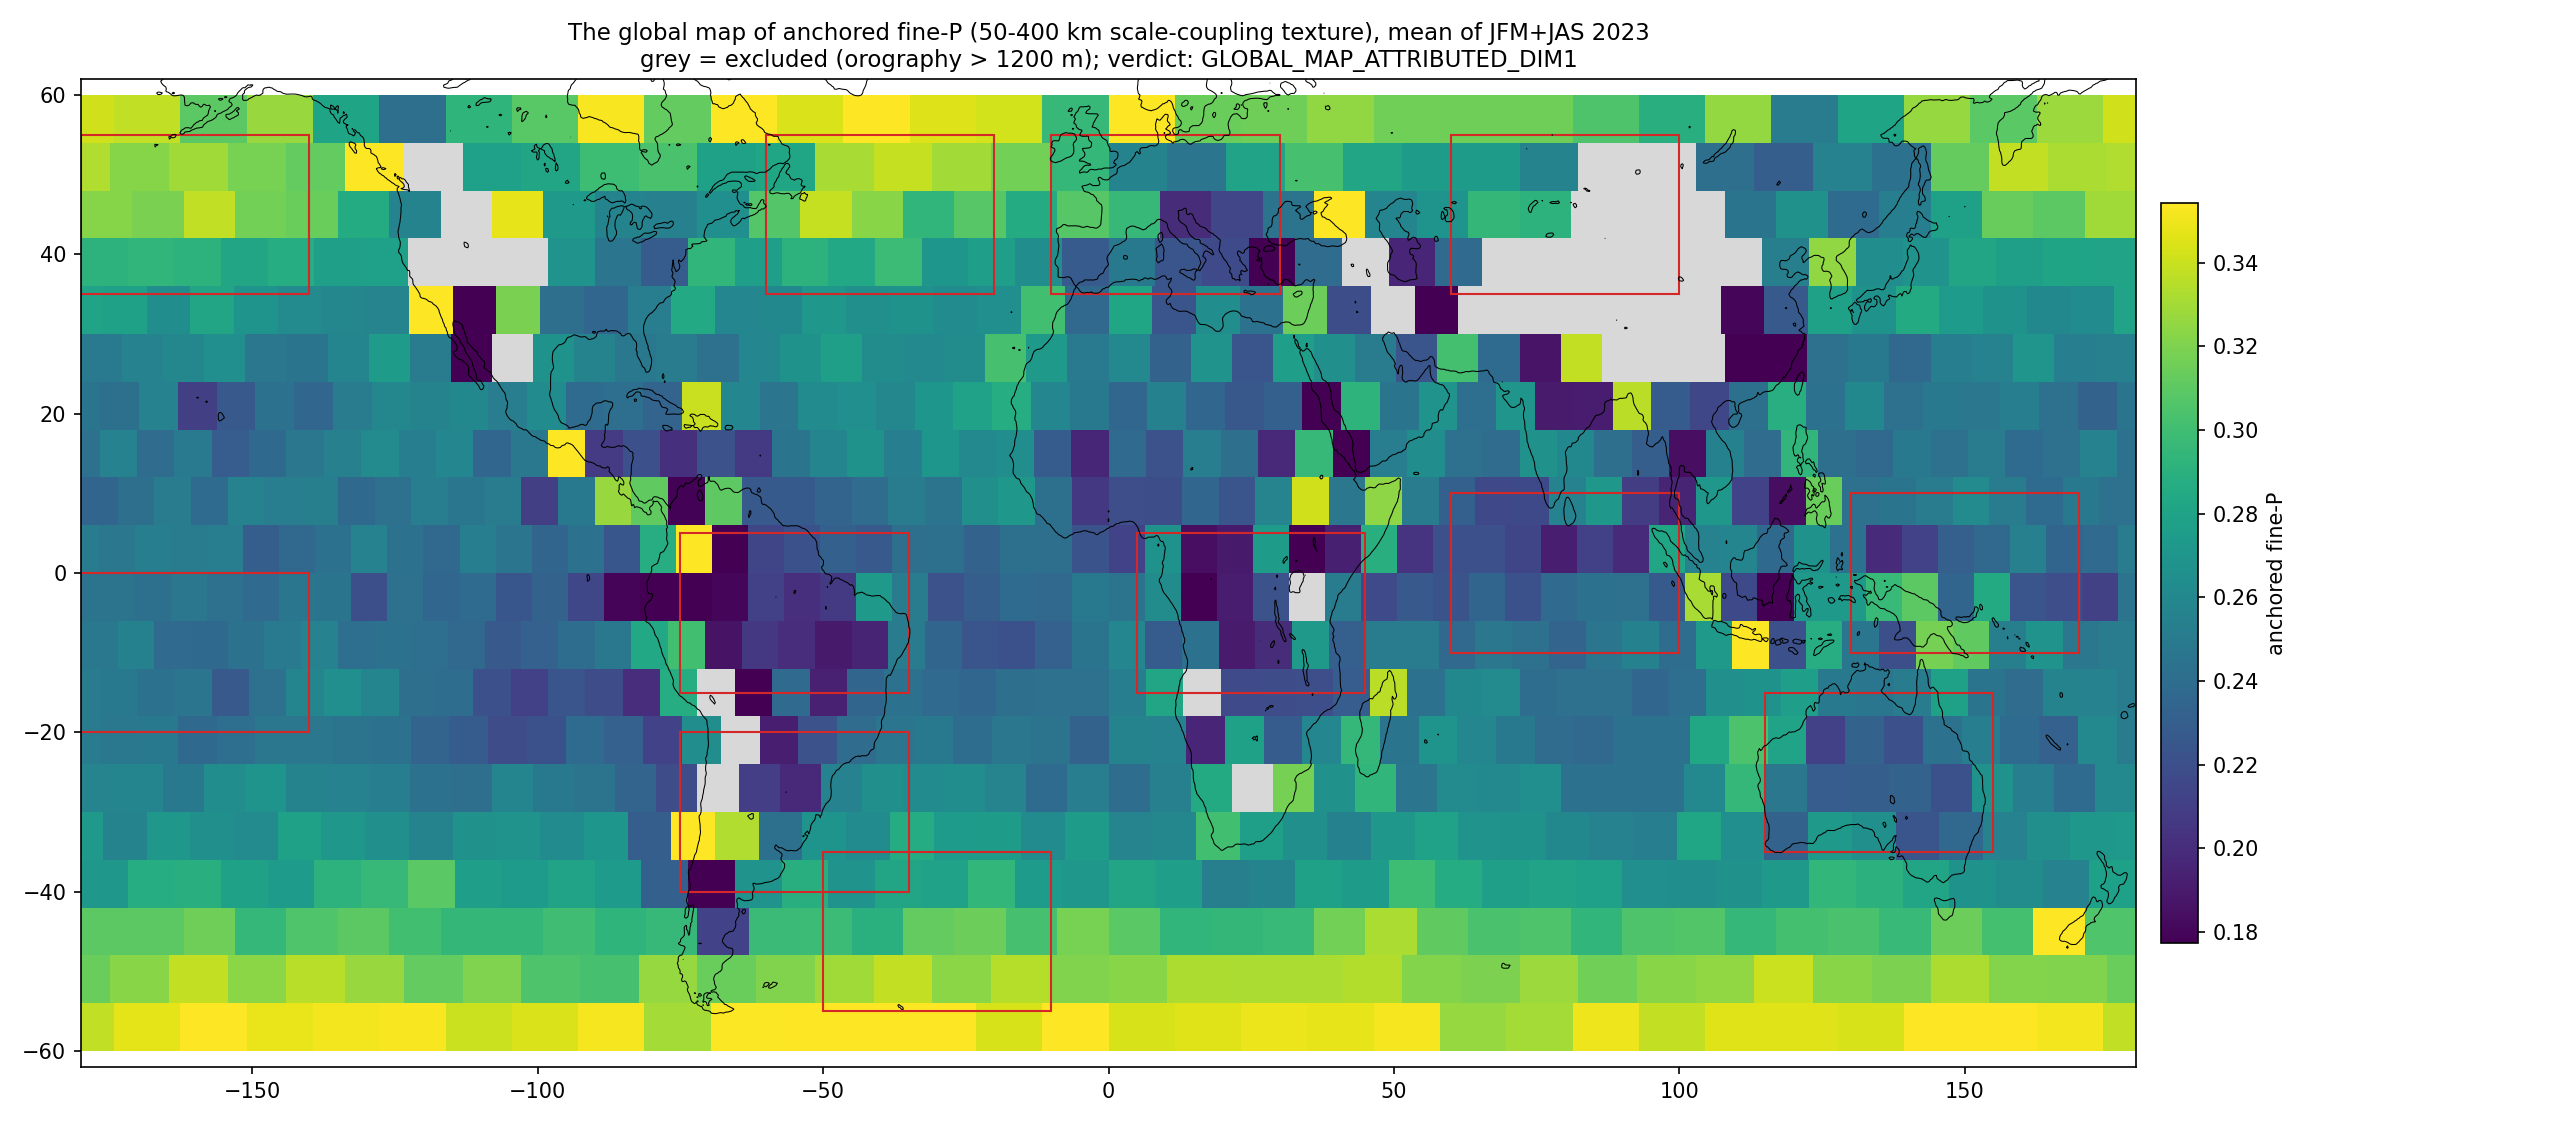
\includegraphics[width=\linewidth]{figures/fig2_global_map.png}

\noindent Рис. 1. Глобальная карта $P$ с суррогатной поправкой (сопряженность полос 50--400 км), среднее сезонов январь--март и июль--сентябрь 2023 г., 936 ячеек, 60$^\circ$ ю.ш.--60$^\circ$ с.ш. Серым -- ячейки, исключенные по орографии (средняя высота более 1200 м); красные рамки -- двенадцать областей программы.

\clearpage
\noindent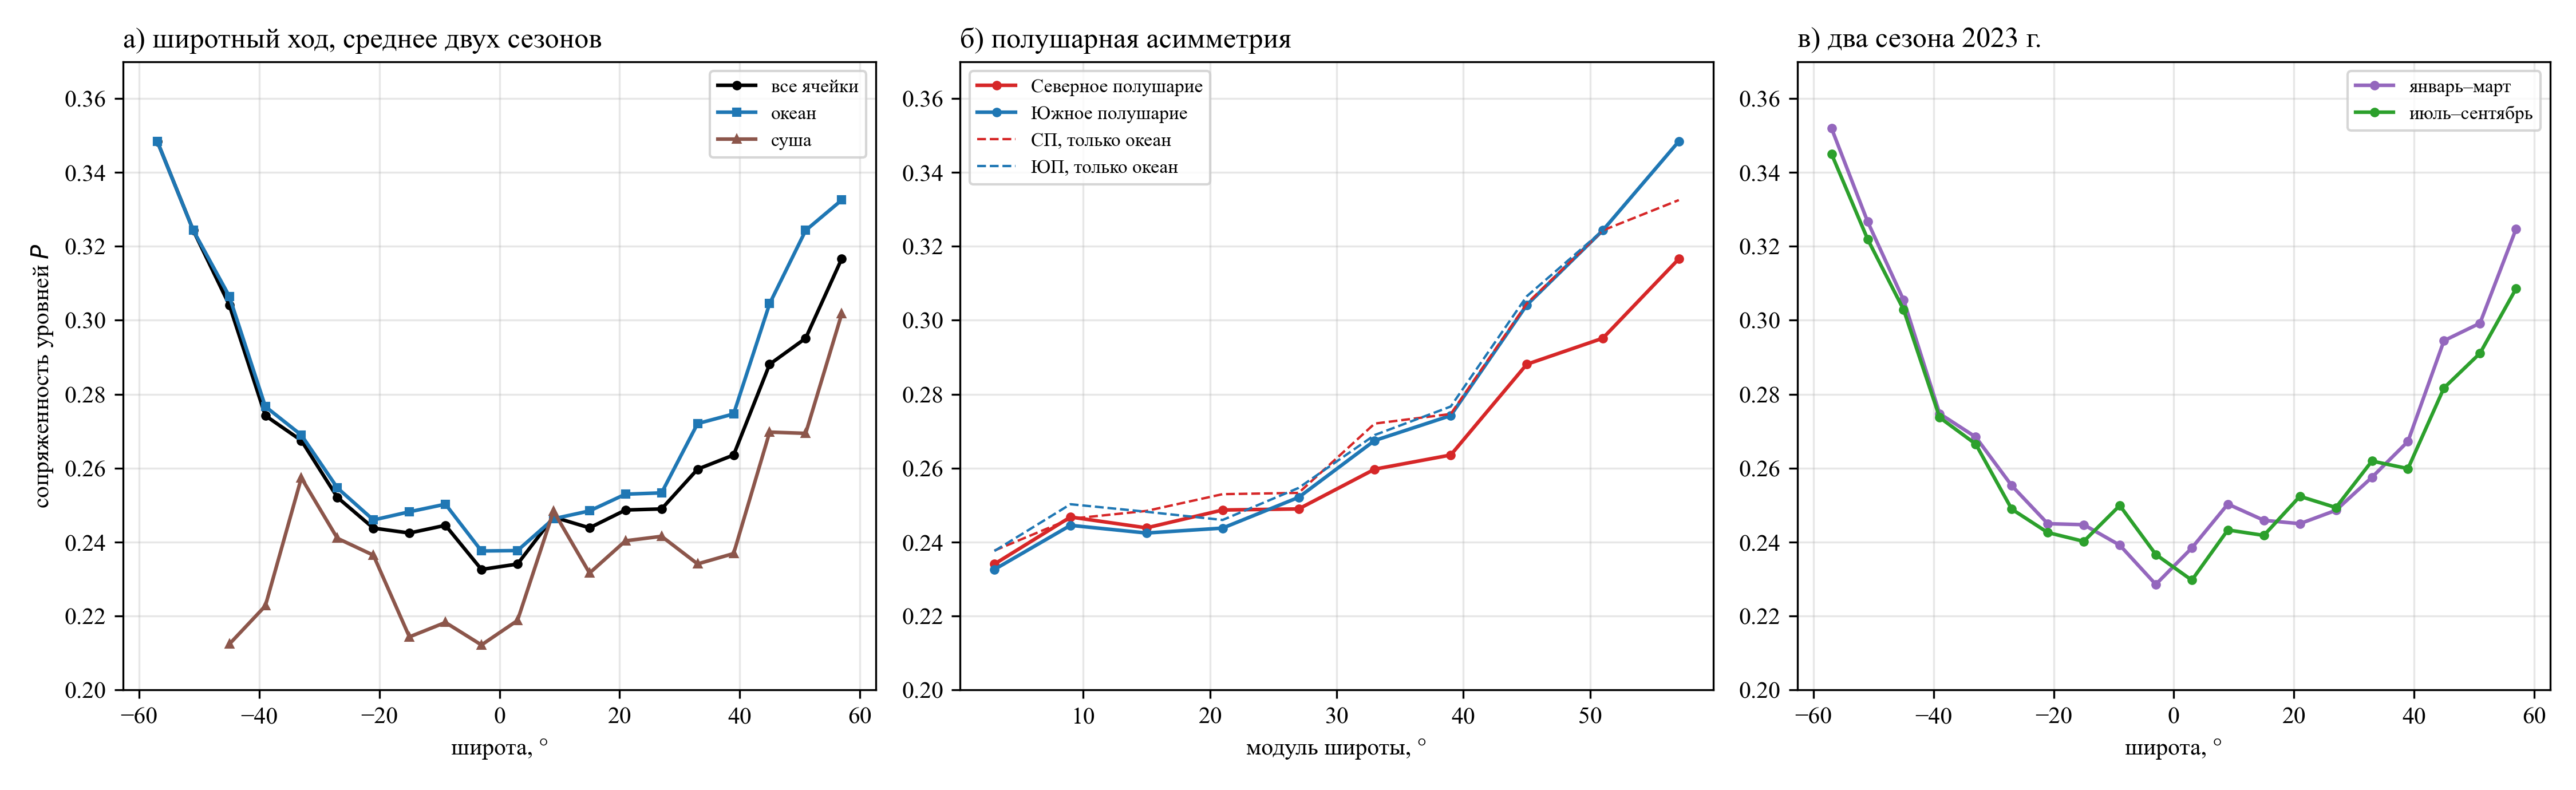
\includegraphics[width=\linewidth]{figures/fig2_zonal_profiles.png}

\noindent Рис. 2. Широтная структура карты (902 ячейки): а -- средние по полосам 6$^\circ$ для всех ячеек, океанических (доля суши менее 0.5) и материковых, среднее двух сезонов 2023 г.; б -- те же средние по модулю широты для Северного и Южного полушарий (сплошные линии -- все ячейки, штриховые -- только океан); в -- широтный ход для сезонов январь--март и июль--сентябрь.

\clearpage
\noindent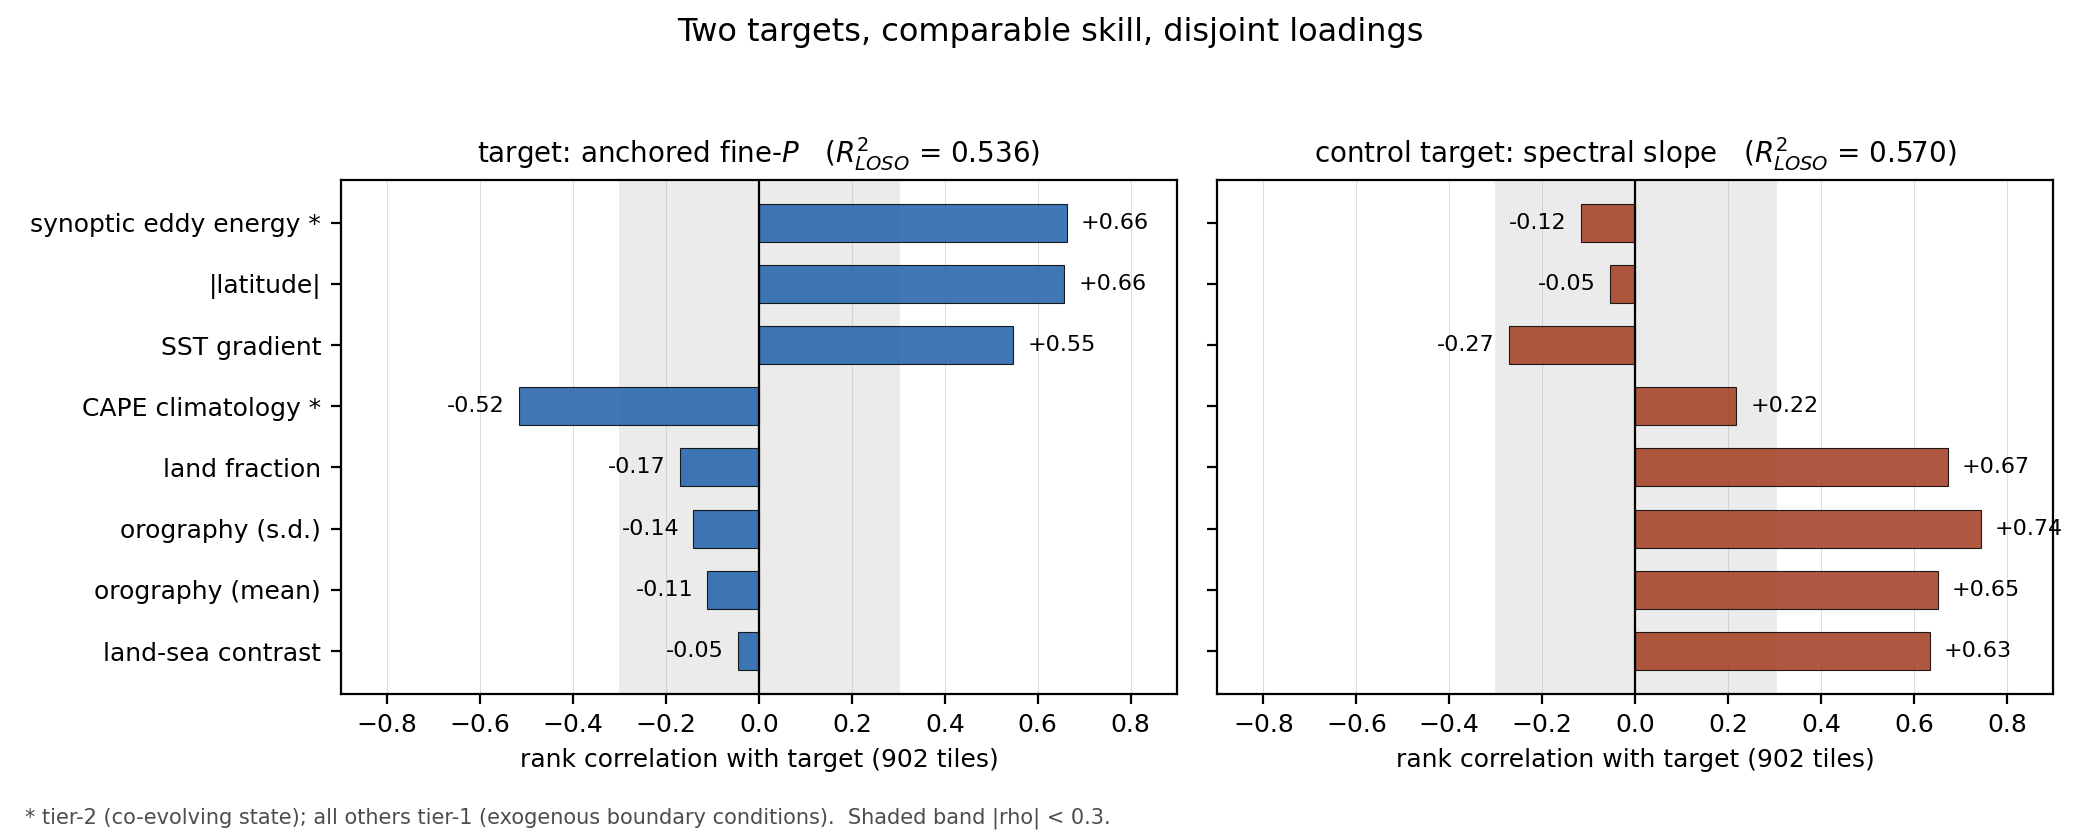
\includegraphics[width=\linewidth]{figures/fig2_channels.png}

\noindent Рис. 3. Двухканальная структура связи: нагрузки восьми ковариат на две мишени глобальной карты -- $P$ с суррогатной поправкой (слева) и наклон пространственного спектра (справа), 902 ячейки. Серая полоса -- диапазон $|\rho| < 0.3$; ведущие ковариаты каждой мишени попадают внутрь этой полосы у другой. Звездочкой помечены характеристики яруса 2.

\clearpage
\noindent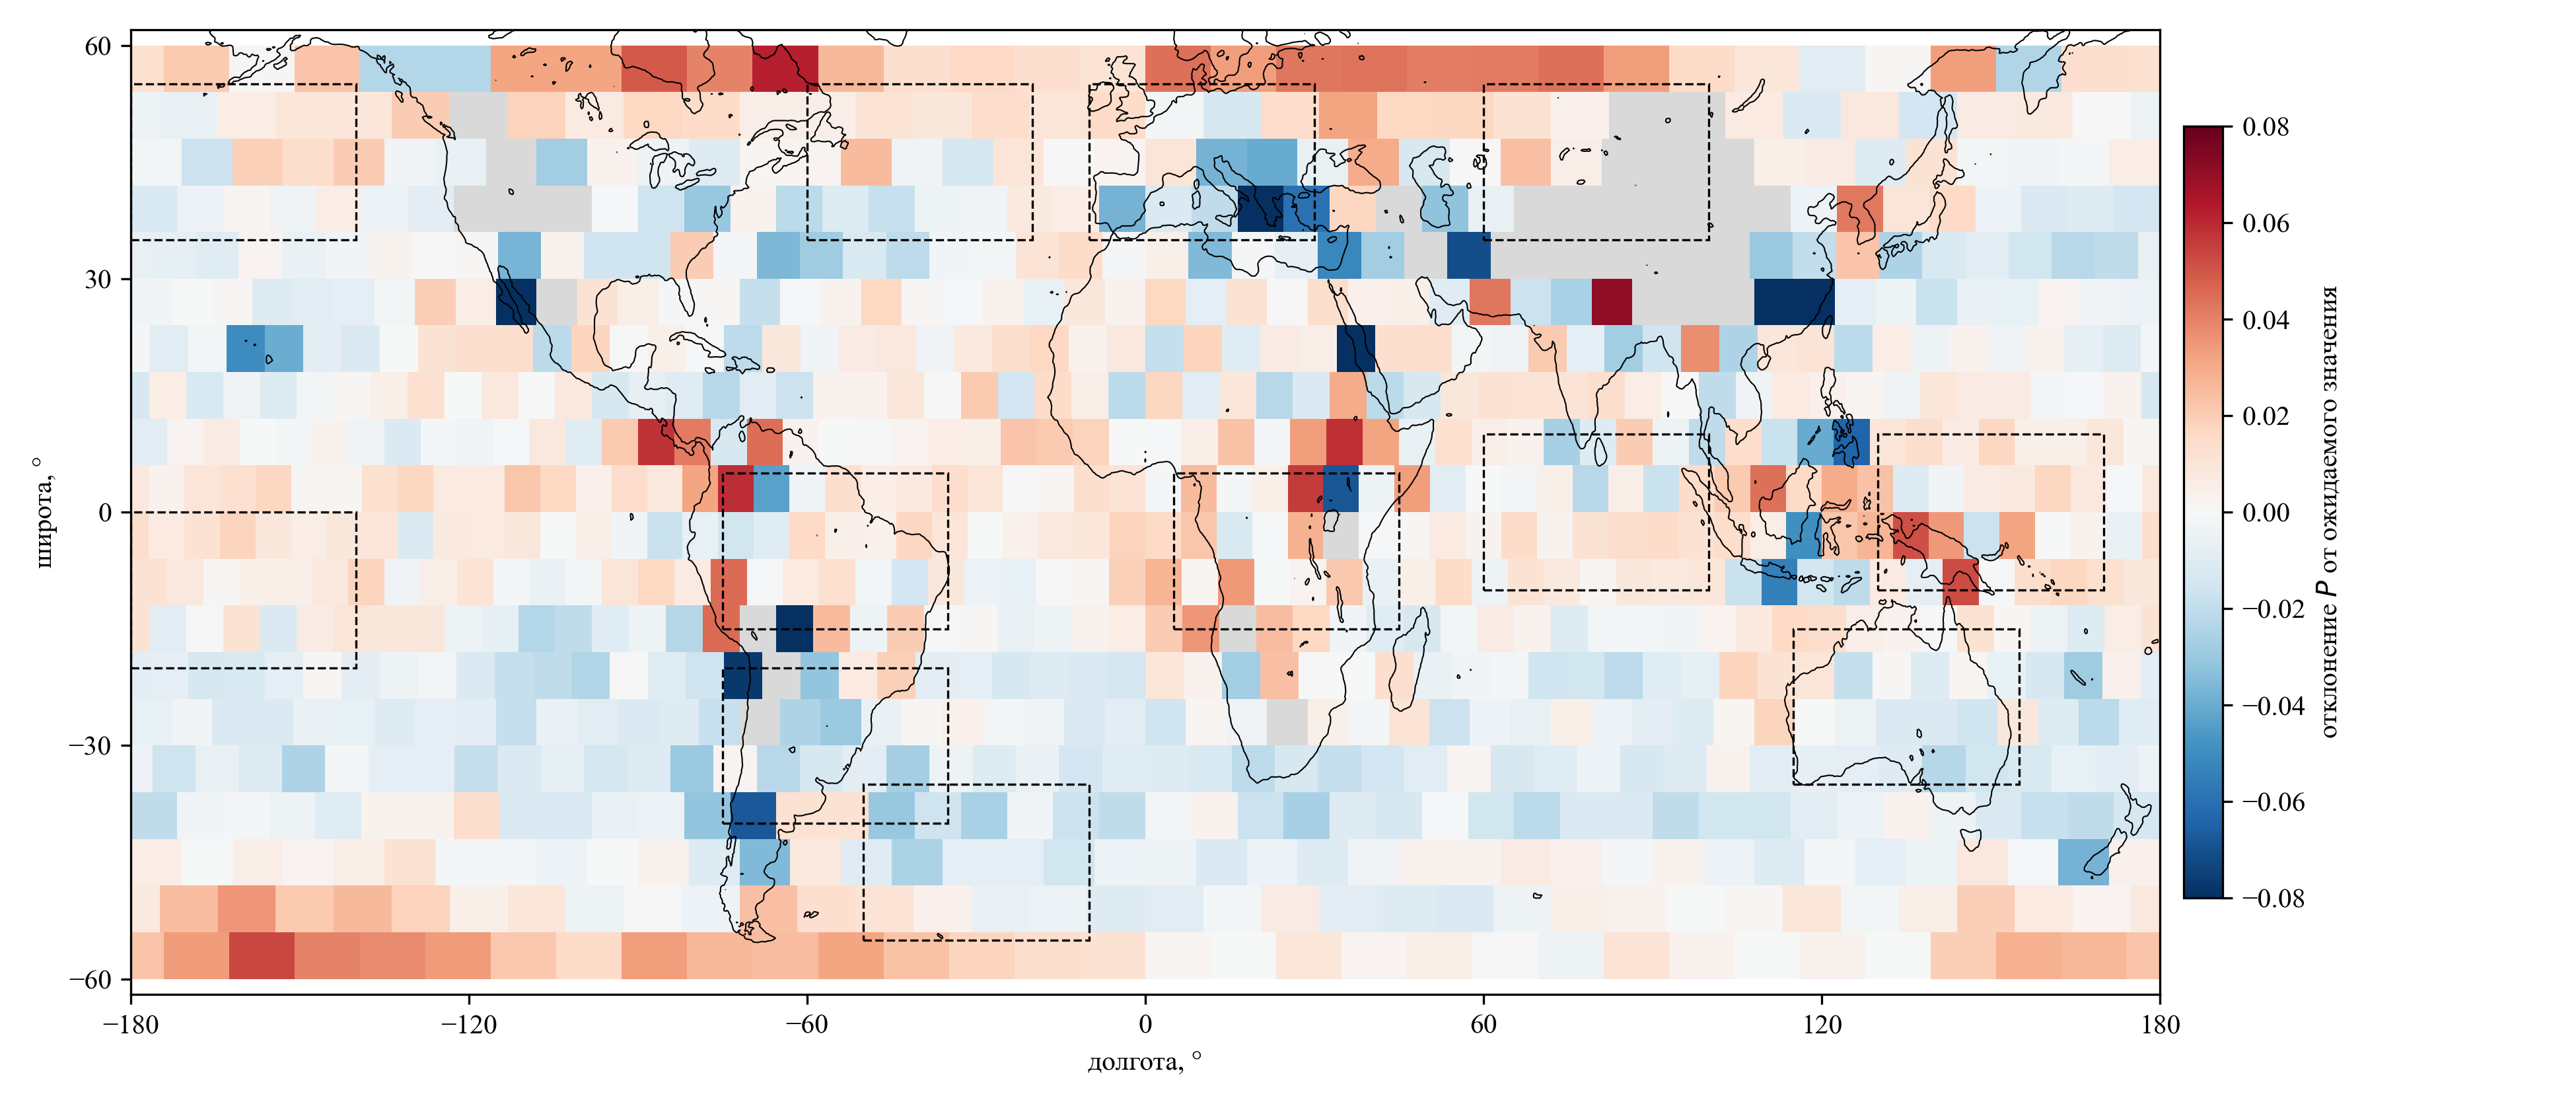
\includegraphics[width=\linewidth]{figures/fig2_residual_map.png}

\noindent Рис. 4. Остаток глобальной карты $P$ после восьми ковариат и блока статистик интермиттентности (среднее двух сезонов 2023 г.; регрессия обучена на противоположной временной половине выборки). Синим -- сопряженность ниже предсказанной (субтропические муссонные окраины, предгорья), красным -- выше (очаги глубокой конвекции, высокоширотные окраины материков). Серым -- ячейки, исключенные по орографии; штриховые рамки -- двенадцать областей программы.

\clearpage
\noindent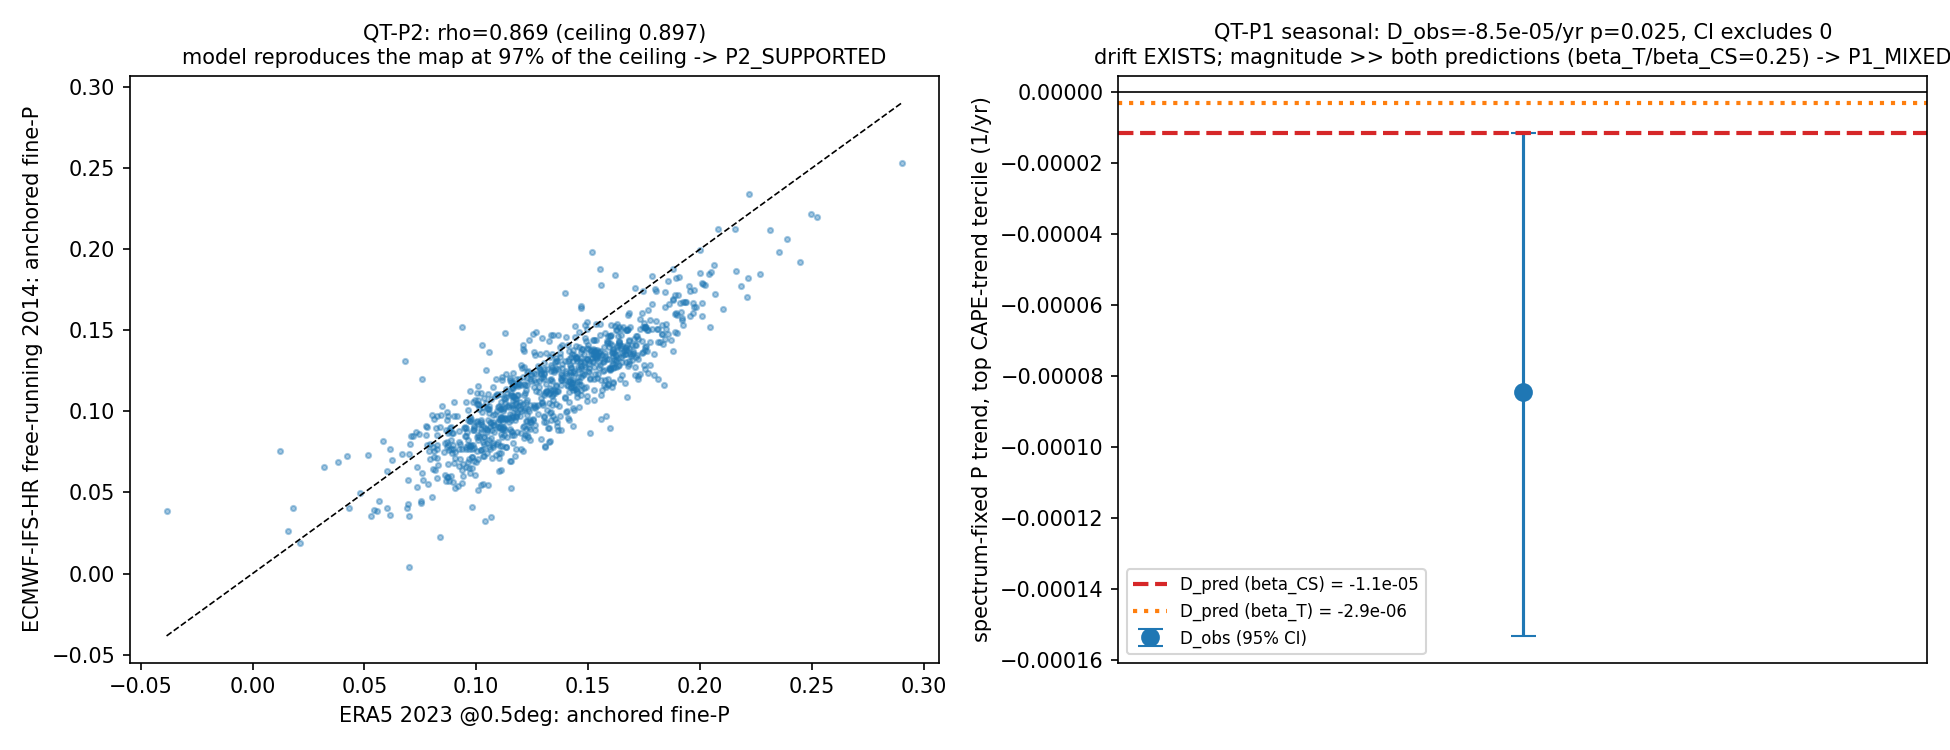
\includegraphics[width=\linewidth]{figures/fig2_qt_round2.png}

\noindent Рис. 5. Слева: карта $P$ свободного расчета ECMWF-IFS-HR (2014 г., без усвоения наблюдений) против карты ERA5 (2023 г.) на 902 согласованных по разрешению ячейках: $\rho = 0.869$ при разрешающем пределе 0.897; пунктир -- линия равенства. Справа: тренд спектрально-фиксированного $P$ в ячейках верхней терцили тренда CAPE (точка -- оценка, отрезок -- 95-процентный доверительный интервал кластерного бутстрэпа) в сравнении с двумя калибровочными предсказаниями (штриховые линии).

\clearpage
\noindent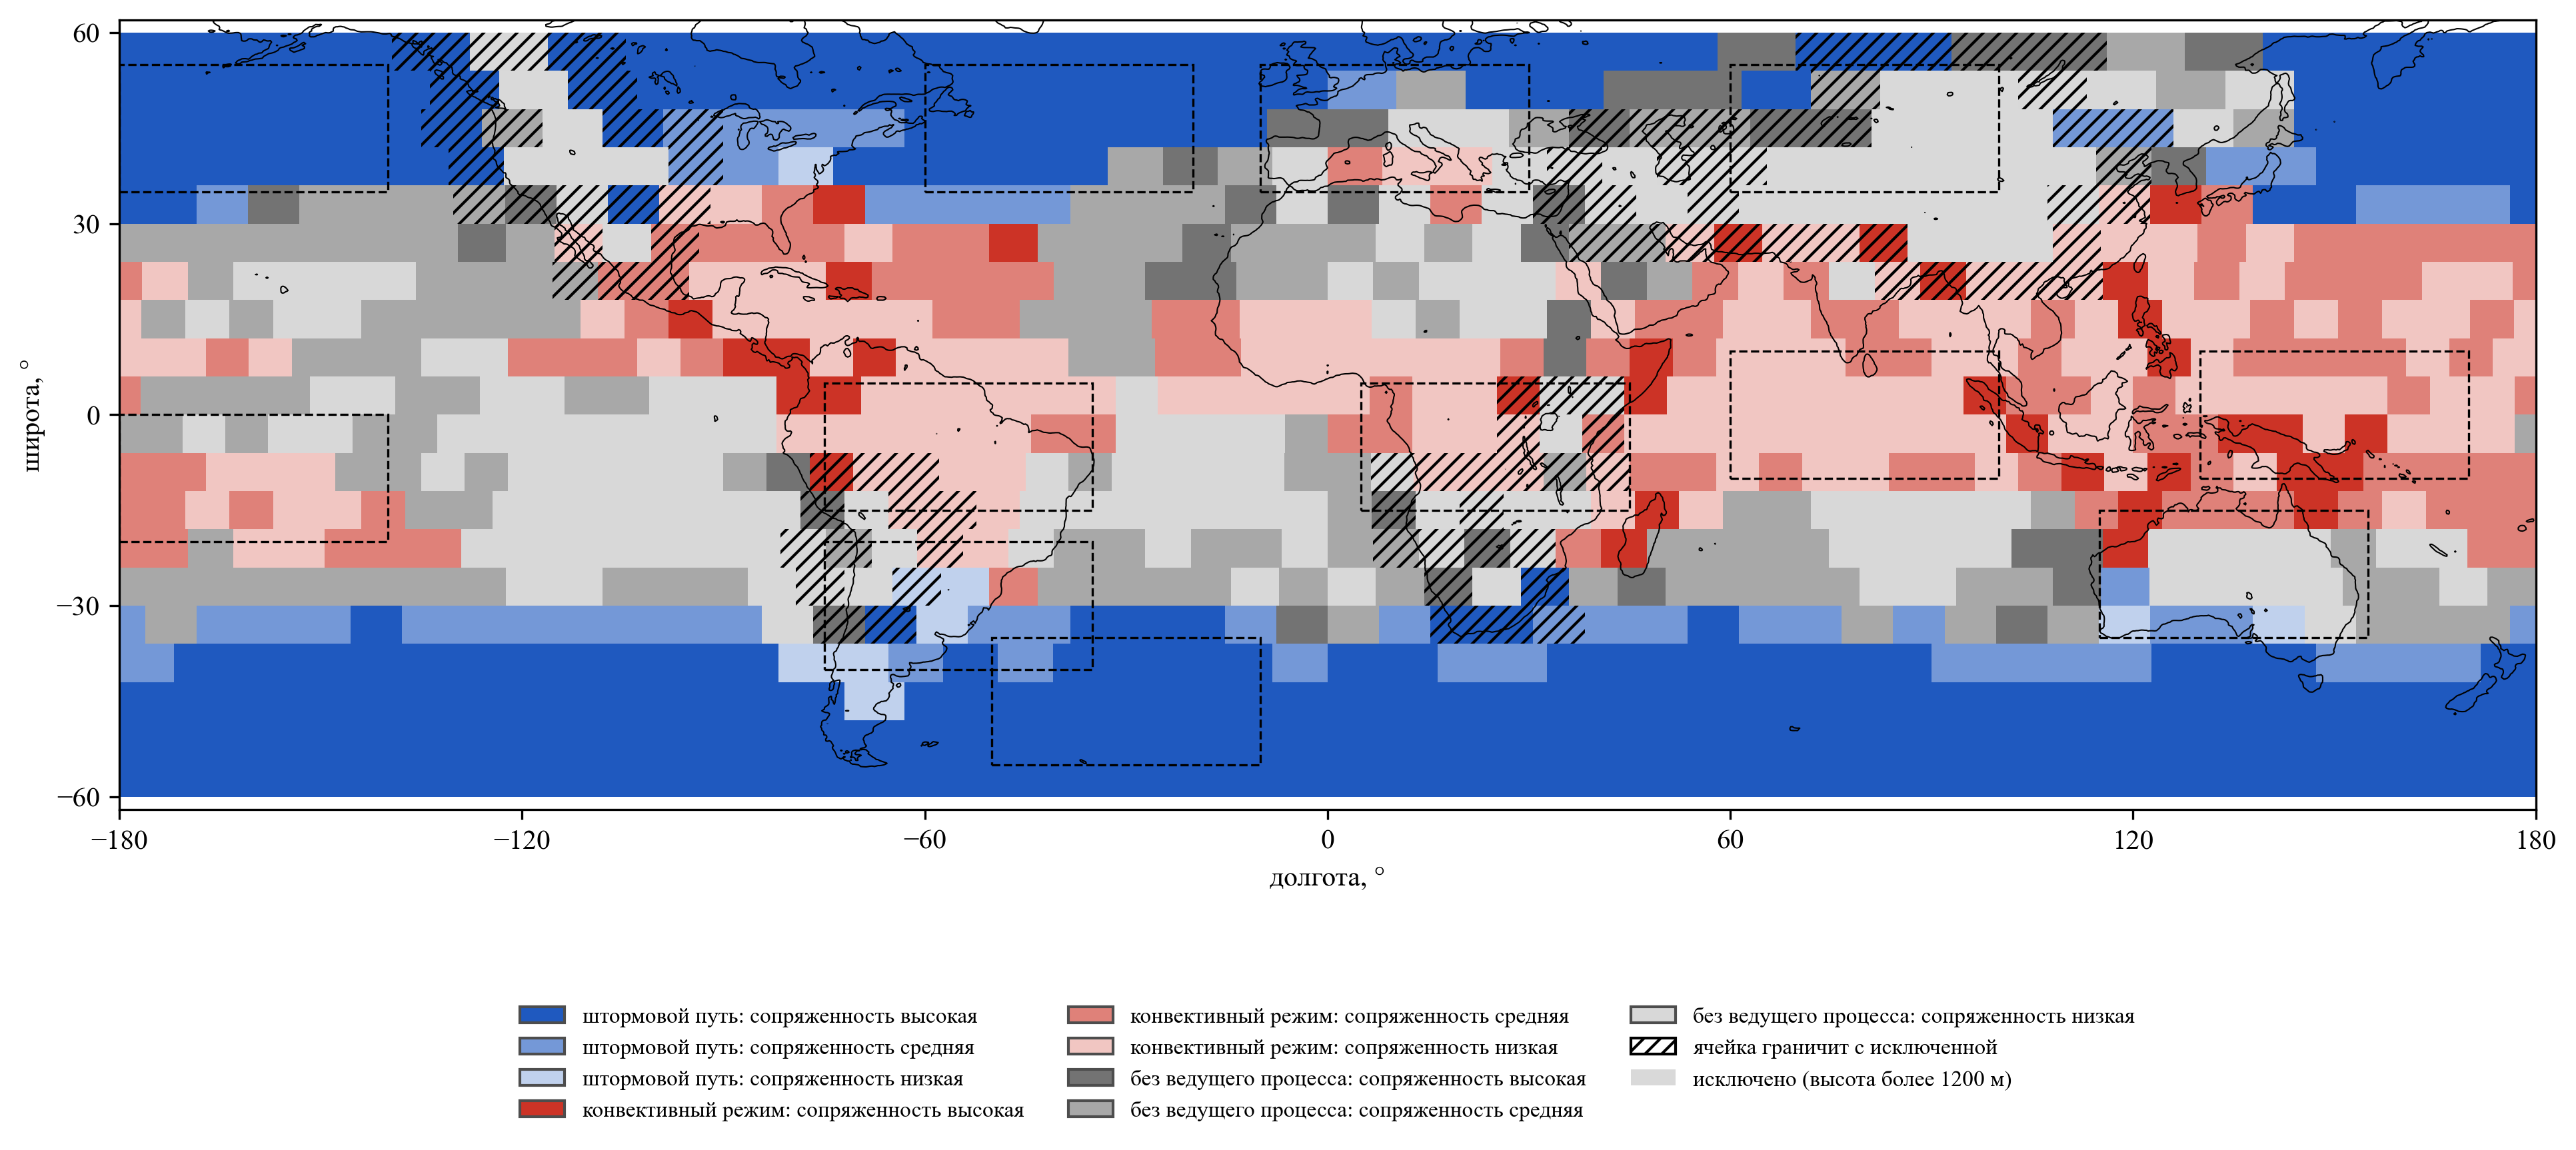
\includegraphics[width=\linewidth]{figures/fig2_regionalization.png}

\noindent Рис. 6. Типология ячеек глобальной карты: цвет -- организатор циркуляции (синий -- штормовой путь, красный -- конвективный режим, серый -- без ведущего организатора), насыщенность -- терциль сопряженности $P$ (темный -- высокая, светлый -- низкая). Штриховка -- ячейки, граничащие с исключенными по орографии; светло-серым -- исключенные; штриховые рамки -- двенадцать областей программы.

\clearpage
\begin{center}
{\large\bfseries Geography of the coupling between hierarchical levels of the atmospheric circulation: a planetary map, its controls and a regionalisation}

\medskip
{\bfseries N. S. Sotiriadi\textsuperscript{*}}

Independent researcher, Moscow, Russia

\textsuperscript{*}E-mail: n.sotiriadi@gmail.com
\end{center}

\begin{singlespace}
\noindent\textbf{Abstract.} The coupling of neighbouring scale levels of the atmospheric circulation -- a measure of how far the placement of mesoscale variability is set by the adjacent large level -- was previously established as a stable regional invariant. This paper asks the geographical question: what is the planetary geography of this invariant and what governs it. From the ERA5 relative-vorticity field at 850 hPa a global mosaic map of 936 tiles of about 667 by 700 km is built between 60$^\circ$S and 60$^\circ$N for two seasons of 2023. The map reads as a physical-geographical one: the maxima form the continuous storm-track ring of the Southern Ocean and the storm tracks of the northern oceans; the minima sit over the deep-convective cores of Amazonia, the Congo basin and the Maritime Continent and over the subtropical monsoon lands. Coupling rises monotonically from the equator to mid-latitudes, is higher over ocean than over land in every belt, and is higher in the Southern than in the Northern mid-latitudes, where the storm track is broken by continents. The tropical seasonal cycle follows the wet season: coupling is lower where and when monsoon convection is active. Attribution on pre-declared covariates confirms this reading: the map is predictable out of sample ($R^2 = 0.40$--$0.54$, $p = 0.001$) and ordered by one axis -- storm-track activity -- while the association is two-channel (storm activity raises coupling through the spectrum, convection lowers it beyond the spectrum), and stationary boundary conditions alone recover 90\% of the predictive skill. A free-running model integration reproduces the map at 97\% of the attainable agreement; the reproducible attribution residual is geographically organised. A typology of territories by circulation organiser and coupling level is proposed as a basis for regionalisation by the architecture of inter-level links.

\smallskip
\noindent\textbf{Keywords:} storm tracks, deep convection, monsoon, reanalysis, free-running model integration, attribution, exogenous boundary conditions, latitudinal zonality, hemispheric asymmetry, typology of territories.

\smallskip
\noindent\textbf{Funding.} The study received no external funding. The author declares no conflict of interest.
\end{singlespace}

\end{document}
